%by AnMnv
\documentclass[a4paper,14pt]{extreport}
\usepackage[left=1.5cm,right=1.5cm,
    top=1.5cm,bottom=2cm,bindingoffset=0cm]{geometry}
\usepackage{scrextend}
\usepackage[T1,T2A]{fontenc}
\usepackage[utf8]{inputenc}
\usepackage[english,russian,ukrainian]{babel}
\usepackage{tabularx}
\usepackage{amssymb}
\usepackage{color}
\usepackage{amsmath}
\usepackage{mathrsfs}
\usepackage{listings}
\usepackage{graphicx}
\graphicspath{ {./images/} }
\usepackage{lipsum}
\usepackage{xcolor}
\usepackage{hyperref}

\usepackage{tcolorbox}
\usepackage{tikz}
\usepackage[framemethod=TikZ]{mdframed}
\usepackage{wrapfig,boxedminipage,lipsum}
\mdfdefinestyle{MyFrame}{%
linecolor=blue,outerlinewidth=2pt,roundcorner=20pt,innertopmargin=\baselineskip,innerbottommargin=\baselineskip,innerrightmargin=20pt,innerleftmargin=20pt,backgroundcolor=gray!50!white}
 \usepackage{csvsimple}
 \usepackage{supertabular}
\usepackage{pdflscape}
\usepackage{fancyvrb}
%\usepackage{comment}
\definecolor{ggreen}{rgb}{0.,1,0}
\definecolor{rred}{rgb}{1,0.1,0.1}
\usepackage{array,tabularx}
\usepackage{colortbl}

\usepackage{varwidth}
\tcbuselibrary{skins}
\usepackage{fancybox}




\usepackage{float}
\usepackage{wrapfig}
\usepackage{framed}





\begin{document}
\pagestyle{plain}
\pagecolor{white}






\begin{titlepage}
  \begin{center}
    \large
    Національний технічний університет України \\ "Київський політехнічний інститут імені Ігоря Сікорського"


    Факультет Електроніки

    Кафедра мікроелектроніки
    \vfill

    \textsc{ЗВІТ}\\

    {\Large Про виконання розрахункової роботи №2\\
      з дисципліни: «Теорія поля»\\[1cm]

   % ДОСЛІДЖЕННЯ ВИПРЯМЛЯЮЧИХ НАПІВПРОВІДНИКОВИХ ДІОДІВ\\

    }
  \bigskip
\end{center}
\vfill

\newlength{\ML}
\settowidth{\ML}{«\underline{\hspace{0.4cm}}» \underline{\hspace{2cm}}}
\hfill
\begin{minipage}{1\textwidth}
Виконавець:\\
Студент 3-го курсу \hspace{4cm} $\underset{\text{(підпис)}}{\underline{\hspace{0.2\textwidth}}}$  \hspace{1cm}А.\,Р.~Півчук\\
\vspace{1cm}

Превірила: \hspace{6.1cm} $\underset{\text{(підпис)}}{\underline{\hspace{0.2\textwidth}}}$  \hspace{1cm}Т.\,А.~Саурова\\

\end{minipage}

\vfill

\begin{center}
2020
\end{center}
\end{titlepage}



%-----------------------------------------------------------------------------------------2-------------------------------------------------------------------------------------------------------------
\begin{center}
\textbf{ЗАВДАННЯ} \\
\end{center}

\textbf{1.} Для коаксіального кабеля з діелектричним заповненням, діаметрами провідників D i d, довжиною l, збудженого на частоті $f$, навантаженого на опір $Z_\text{н}$, розрахувати КСХ, коефіціент відбивання і вхідний опір. Побудувати графіки розподілу амплітуд струму і напруги вздовж кабеля.\par

\textbf{2.} Розрахувати місце підключення та величину реактивності (наприклад, довжину шлейфа), необхідної для узгодження лінії з даним навантаженням.\\


\begin{center}
\vspace{0.1cm}

\begin{tabular}{ | c |  c |  c |  c |}
\hline
вар. № & 4   \\
\hline
$\varepsilon \text{(фторопласт)}$ & 2.0   \\
\hline
$f, $ ГГц& 2   \\
\hline
$D, $ мм&  0.41  \\
\hline
$d, $ мм&  2.2  \\
\hline
$l, $ cм& 40   \\
\hline
$\dot{Z_{H}}, $ Ом & 25-i25   \\
\hline
\end{tabular}
\vspace{0.2cm}
\end{center}




%--------------------------------------------------------------------------------3----------------------------------------------------------------------------------------------------------------------
\newpage
\begin{center}
\textbf{РОЗРАХУНКИ} \\
\end{center}

Оскільки, на низьких частотах немає особливих проблем об'єнання електронних компонентів у кола за допомогою звичайних провідників, але на високих частотах, коли довжина провідників стає співмірною з довжиною хвилі сигналу, через скінченність часу розповсюдження електромагнітного збудження потенціал у різних точках вздовж провідника буде різним. За цих умов стають невірними закони Ома та Кірхгофа, на яких заснована теорія кіл, і точний аналіз процесів тут можливий тільки на основі теорії поля. Тому припускаємо що погонна провідність та погонний опір є незначним ($r_{0}\ll\omega L_{0} , g_{0}\ll\omega C_{0}$) і ми маємо справу з лінією без втрат. \par

Спочатку знайдемо всі параметри які потрібні для розрахунку значення хвильового опору:
\begin{equation}\label{eq1}
\dot{Z_{0}} = \sqrt{\dfrac{L_{0}}{C_{0}}},
\end{equation}
де $L_{0}$ -- погонна індуктивність та $C_{0}$ -- погонна ємність.

\begin{equation}\label{eq2}
L_{0} = \dfrac{\mu\mu_{0}\cdot ln\dfrac{D}{d}}{2\pi},
\end{equation}
де $D$ та $d$ -- зовнішній та внутрішній діаметр відповідно; $\mu$ -- магнітна проникність середовища; $\mu_0$ -- магнітна стала.


\begin{equation}\label{eq3}
C_{0} = \dfrac{2\pi \varepsilon \varepsilon_0}{ln\cdot\dfrac{D}{d}},
\end{equation}
де $\varepsilon_0$ -- діелектрична стала; $\varepsilon$ -- діелектрична проникність середовища. \\

Підставляючи отримаємо:
\begin{equation}\label{eq4}
\dot{Z_{0}} =\sqrt{ \dfrac{\dfrac{\mu\mu_{0}\cdot ln\dfrac{D}{d}}{2\pi}}{\dfrac{2\pi \varepsilon \varepsilon_0}{ln\cdot\dfrac{D}{d}}}}
=\sqrt{\dfrac{\mu\mu_{0}\cdot ln\dfrac{D}{d}}{2\pi}\cdot \dfrac{ln\cdot\dfrac{D}{d}}{2\pi \varepsilon \varepsilon_0}} = \dfrac{ln\dfrac{D}{d}}{2\pi}\sqrt{\dfrac{\mu\mu_{0}}{ \varepsilon \varepsilon_0} },
\end{equation}
оскільки поліетилен є дієлектриком, то $\mu = 1$ та знаючи що $\sqrt{\dfrac{\mu_{0}}{\varepsilon_0}} = 120\pi$, тоді

\begin{equation}\label{eq5}
\dot{Z_{0}} = \dfrac{ln\dfrac{D}{d}}{2\pi} \cdot \sqrt{\dfrac{1}{\varepsilon}} \cdot 120\pi = 73.0382\approx 73 \text{ Ом}
\end{equation}



%-----------------------------------------------------------------------------------------4------------------------------------------------------------------------------------------------------------
Припускаємо що $r_{0} =0 , g_{0} = 0$, тобто маємо ідеальний діелектрик і лінію без втрат, тому можна вивести формулу для розрахукну хвильового числа (характеризує зміну фази хвилі на одиницю довжини):
\begin{align}\label{eq6}
V_{\text{ф}} = \dfrac{\omega}{k} = \dfrac{1}{\sqrt{L_0C_0}} \hspace{0.5 cm} \Rightarrow \hspace{0.5 cm} k = \omega\sqrt{L_0C_0},
\end{align}
де $\omega=2\pi f$ -- кругова частота часових коливань, що показує зміну фази за одиницю часу.
\begin{align}\label{eq78}
k =  2\pi f \cdot \sqrt{\dfrac{\mu\mu_{0}\cdot ln\dfrac{D}{d}}{2\pi} \cdot \dfrac{2\pi \varepsilon \varepsilon_0}{ln\cdot\dfrac{D}{d}} }=
\mu2\pi f\sqrt{\mu_0\varepsilon_0\varepsilon}\\
k = \dfrac{2\pi f \sqrt{\varepsilon}}{c} = 31 \text{ м}^{-1}, \text{ врахувавши що } \mu = 1 \text{ та } \sqrt{\mu_0\varepsilon_0} = \dfrac{1}{c}
\end{align}

\begin{center}
Доведемо що наша лінія дійсно є довгою
\end{center}
\begin{align*}\label{eq0.1}
\lambda = \dfrac{2\pi}{k} = \dfrac{2\cdot 3.14}{31} = 0.2 \hspace{0.2 cm} \text{м}\hspace{0.2 cm} \Rightarrow \hspace{0.2 cm }\lambda \textless l
\end{align*}
\vspace{0.2cm}
Наступним кроком розрахуємо  \colorbox{cyan}{коефіціент відбивання} $\dot{\rho}$\footnote[1]{$\dot{\rho} = |\dot{\rho}| \cdot e^{i\varphi_0}\hspace{0.2 cm } \Rightarrow\hspace{0.2 cm }  \varphi_0 = 1.5$} :
\begin{equation}\label{eq9}
\resizebox{.9\textwidth}{!}{%
$ \dot{\rho}= \dfrac{\dot{Z_H} - \dot{Z_0} }{\dot{Z_H} + \dot{Z_0}} = \dfrac{50-i50 - 73}{50-i50 + 73} = \dfrac{-23-i50}{123-i50} =\dfrac{55\cdot e^{iarctg\left(\dfrac{50}{23}\right)}}{132.7\cdot e^{iarctg\left(-\dfrac{50}{123}\right)}} =  0.41\cdot e^{i\cdot arctg(77)} =  0.41\cdot e^{i\cdot 1.5}$}%
\end{equation}
\begin{align}\label{eq10}
\colorbox{green}{КСХ}= \dfrac{1+|\dot{\rho}|}{1-|\dot{\rho}|} = \dfrac{1+|0.41|}{1-|0.41|} = 2.38
\end{align}
Для розрахунків розподілу амплітуд струму та напруги вздовж кабеля, використаємо нормування:
\begin{align}\label{eq11}
V_m(x) = V_m^+|1+|\dot{\rho}|\cdot e^{-i(2kx-\varphi_0)}  |
\end{align}
\begin{align*}
\dfrac{V_m(x)}{V_m^+} &= |1+|\dot{\rho}|\cdot e^{-i(2kx-\varphi_0)}| = |1+|\dot{\rho}|\cdot cos(2kx-\varphi_0)| - |{\rho}| \cdot i \cdot \sin(2kx-\varphi_0)| =\\
&= \sqrt{(1+0.41\cdot cos(62x-1.5))^2 - (0.41 \cdot i \cdot \sin(62x-1.5))^2} = \\
&=\sqrt{1+0.82\cdot cos(62x-1.5) + 0.1681}
\end{align*}



%-----------------------------------------------------------------------------------------5------------------------------------------------------------------------------------------------------------
\begin{align}\label{eq12}
I_m(x) = I_m^+|1-|\dot{\rho}|\cdot e^{-i(2kx-\varphi_0)}|
\end{align}
\begin{align*}
I_m(x) &= I_m^+|1+|\dot{\rho}|\cdot e^{-i(2kx-\varphi_0)}  |\\
\dfrac{I_m(x)}{I_m^+} &= |1-|\dot{\rho}|\cdot e^{-i(2kx-\varphi_0)}| = |1-|\dot{\rho}|\cdot cos(2kx-\varphi_0)| - |{\rho}| \cdot i \cdot \sin(2kx-\varphi_0)| =\\
&= \sqrt{(1-0.41\cdot \cos(62x-1.5))^2 - (0.41 \cdot i \cdot \sin(62x-1.5))^2} = \\
&=\sqrt{1-0.82\cdot \cos(62x-1.5) + 0.1681}
\end{align*}


\begin{figure}[h]
\center{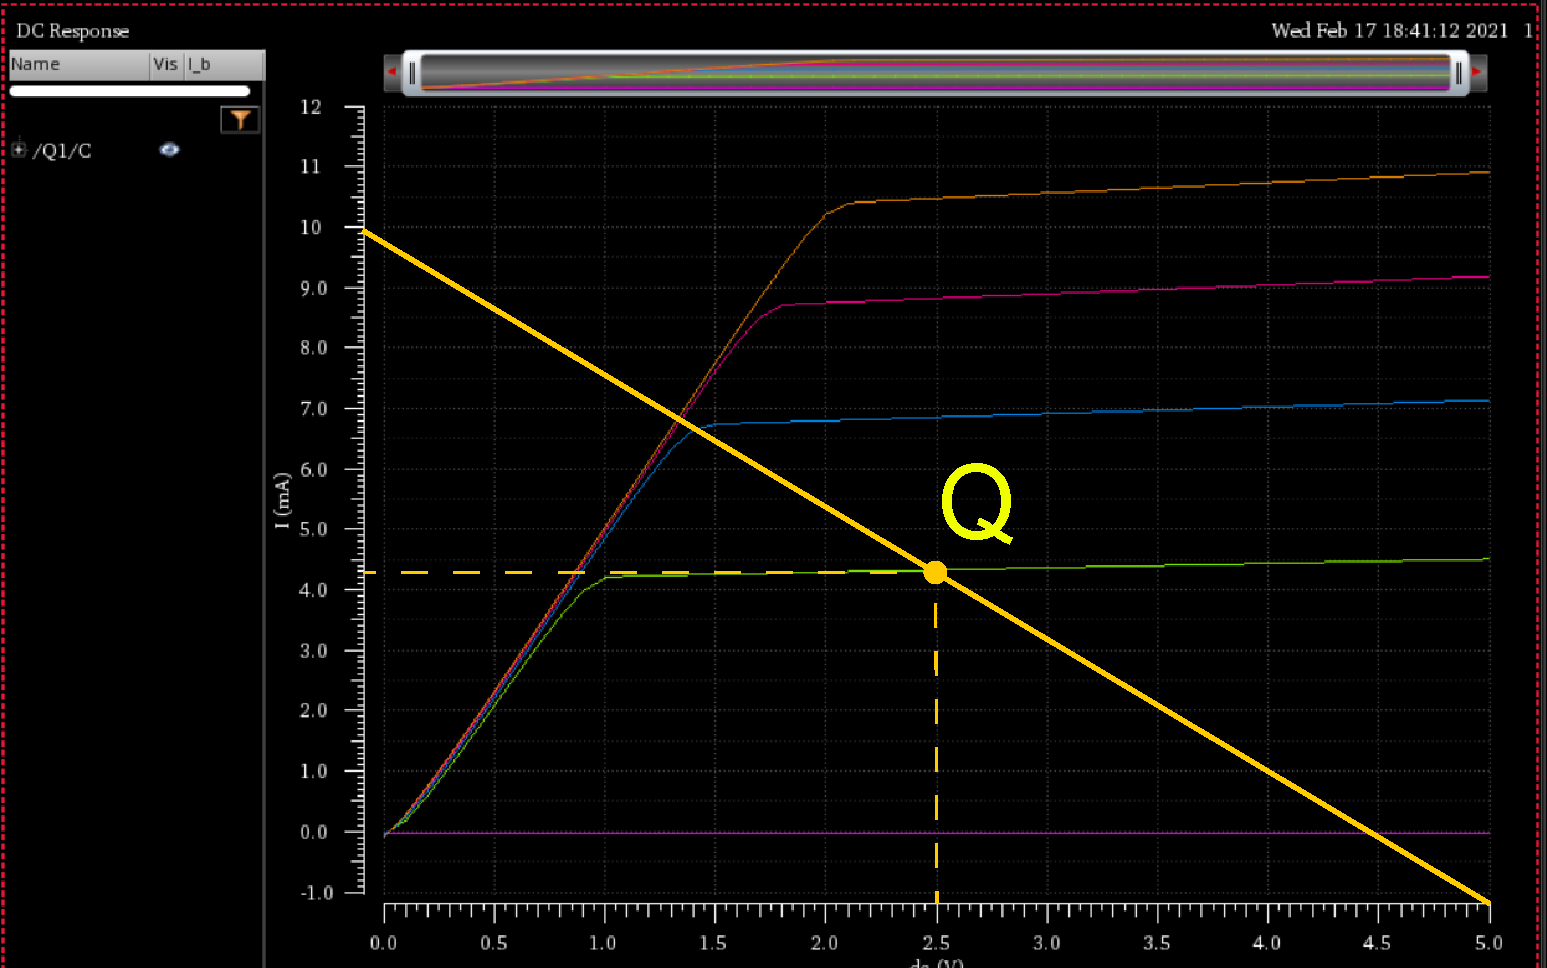
\includegraphics[width=1\linewidth]{1.pdf}}
\caption{Розподіл амплітуд напруги та струму вздовж напруги.}
\label{ris:image1}
\end{figure}


У випадку за нерівності опору навантаження і хвильового опору, як в данному випадку $\dot{Z}_H\neq \dot{Z}_0$, в лінії встановлюється режим змішаних хвиль, який можна розглядати як суперпозицію режимів біжучої і чисто стоячої хвилі. Тому опір вздовж лінії буде змінюватися відповідно за законом:
\begin{align}\label{eq13}
\dot{Z}(x) = \dot{Z}_0\dfrac{\dot{Z}_H + i\cdot Z_0\cdot tg (kx)}{Z_0 + i\cdot \dot{Z}_H\cdot tg (kx)}
\end{align}
%-----------------------------------------------------------------------------------------6-------------------------------------------------------------------------------------------------------------

Нехай початок координат буде у місці підключення навантаження. Тоді $\dot{Z}(x) = \dot{Z}(l) = \dot{Z}_{\text{вх}}$, тому \colorbox{pink}{вхідний опір}:
\begin{align}\label{eq14}
\dot{Z}_{\text{вх}} = Z_0 \cdot\dfrac{\dot{Z}_H + i\cdot Z_0\cdot tg (kl)}{Z_0 + i\cdot \dot{Z}_H\cdot tg (kl)}
\end{align}
\begin{align*}
\dot{Z}_{\text{вх}} &= 73\cdot \dfrac{50-50i + i\cdot 73\cdot tg (31\cdot 1)}{73 + i\cdot (50-50i)\cdot tg (31\cdot 1)}
 			    = 73\cdot \dfrac{50-50i + 0.6i}{73 + (50-50i)\cdot 0.6i}=\\
			    &= 73\cdot \dfrac{50-17i}{73 + (50-50i)\cdot 0.6i}=73\cdot \dfrac{50-17i}{103 + 30i} = \dfrac{3650-1241i}{103 + 30i} = 32.6 - 9.5i
\end{align*}

Тепер знайдемо величину і місце підключення шлейфу, для цього використовуємо режим змішаних хвиль.
Нехай $x^*$ -- місце підключення шлейфа:
\begin{align}\label{eq15}
\dot{Z}(x^*) = Z_0 \pm iX(x^*)
\end{align}
\begin{align}\label{eq16}
Re\dfrac{\dot{Z}_H + i\cdot Z_0\cdot tg (kx^*)}{Z_0 + i\cdot \dot{Z}_H\cdot tg (kx^*)} = 1\hspace{0.5 cm}
Re\left(\dfrac{50-i50 + i\cdot 73\cdot tg (31x^*)}{73 + i\cdot (50-i50)\cdot tg (31x^*)}\right) = 1
\end{align}

\begin{align*}
\resizebox{.9\textwidth}{!}{%
$\dfrac{50-i50 + i\cdot 73\cdot tg (31x)}{73 + i\cdot (50-i50)\cdot tg (31x)} =
\dfrac{(50-i50 + i\cdot 73\cdot tg (31x))\cdot (73+50\cdot tg (31x)-i\cdot 50\cdot tg(31x))}{ (73+50\cdot tg (31x)+i\cdot 50\cdot tg(31x)) \cdot  (73+50\cdot tg (31x)-i\cdot 50\cdot tg(31x))} =$
}
\end{align*}
\begin{align*}
=\dfrac{73\cdot 50 + 50\cdot50tg(31x)+ 50\cdot50tg(31x)+ 73+50tg^2(31x)}{(73+50tg(31x))^2 - (50itg(31x)))^2} +
\end{align*}
\begin{align*}
\resizebox{.9\textwidth}{!}{%
$+ \dfrac{-50i\cdot50tg(31x) - 50 \cdot 73i-50\cdot50tg(31x)\cdot i + 73\cdot73tg(31x)\cdot i + 73\cdot50tg^2(31x)\cdot i}{(73+50tg(31x))^2 - (50itg(31x)))^2}$}
\end{align*}


Видокремивши реальну частину можна розв'язати наступне рівняння:
\begin{align*}
\resizebox{.9\textwidth}{!}{%
$ \dfrac{73\cdot 50 + 50\cdot50tg(31x) +50\cdot50tg(31x)+ 73\cdot50tg^2(31x) }{(73+50tg(31x))^2 - 2500tg^2(31x)} = 1$}
\end{align*}
\begin{align*}
\resizebox{.9\textwidth}{!}{%
$ 3650+ 5000\cdot tg(31x) + 3650\cdot tg^2(31x) = 5329 +7300 \cdot tg(31x) + 2500 \cdot tg^2(31x) -2500 \cdot tg^2(31x)$}
\end{align*}
\begin{align*}
\resizebox{.9\textwidth}{!}{%
$ 1679+2300\cdot tg(31x) - 3650\cdot tg^2(31x) =  0$}
\end{align*}
Корені рівняння:
\begin{align*}
 x_1& = \dfrac{-2300+10\sqrt{298034}}{2\cdot(-3650)} = -0.432\\
x_2 &= \dfrac{-2300-10\sqrt{298034}}{2\cdot(-3650)} = 1.062\\
\end{align*}
\newpage


%-------------------------------------------------------------------------------------7-----------------------------------------------------------------------------------------------------------------
\begin{align*}
31x &= arctg(-0.432) + \pi k
\end{align*}

\begin{align*}
 x_1& = \dfrac{arctg(-0.432)}{31} \textless 0\\
  x_2& =  \dfrac{arctg(-0.432)+\pi}{31} = 2.76 = 0.089\\
   x_3& =  \dfrac{arctg(1.062)+\pi}{31} = 0.814 = 0.026 \text{ --- найменше додатнє значення} \Rightarrow x^* = 0.026\\
    x_4& =  \dfrac{arctg(1.062)+\pi}{31} = 4 = 0.12
\end{align*}
Знайшовши точку піжключення шлейфа, $x^* = 0.026$, тепер можна розрахувати величену реактивності за наступною формулою:
\begin{align}
X(x^*) = -iIm(\dot{Z}(x^*))
\end{align}
Підставивши замість x величину $x^*$ отримаємо:
\begin{align}
\resizebox{.9\textwidth}{!}{%
$-i\cdot Im(\dot{Z}(x^*)) =  \dfrac{-50\cdot50tg(31x) - 50 \cdot 73-50\cdot50tg(31x) + 73\cdot73tg(31x) + 73\cdot50tg^2(31x)}{(73+50tg(31x))^2 + (50tg(31x))^2}$}
\end{align}

Реактивний опір і положення шлейфу можна знайти графічно, побудувавши функції $Re(\dot{Z}(x^*))$ та $Im(\dot{Z}(x^*))$, графічно знаходимо точку $x^*$ в якій $Re(\dot{Z}(x^*))= Z_0 = 73$Ом а з другого графіку знаходимо значення реактивного опору $X(x^*)$ у цій же просторовій точці.


%\begin{align}
%X(x^*) = -i \cdot \dfrac{244671}{1984.4} =  -i \cdot (-12.3) = 12.3\cdot i
%\end{align}
%Оскільки  $X(x^*)$> 0 то реактивний опір має індуктивний  характер. І можна розрахувати цю індуктивність шлейфу з формули:



%----------------------------------------10--------------------------------------------------------------------------------------------------------------------------------------------------------------
\newpage
\begin{figure}
\center{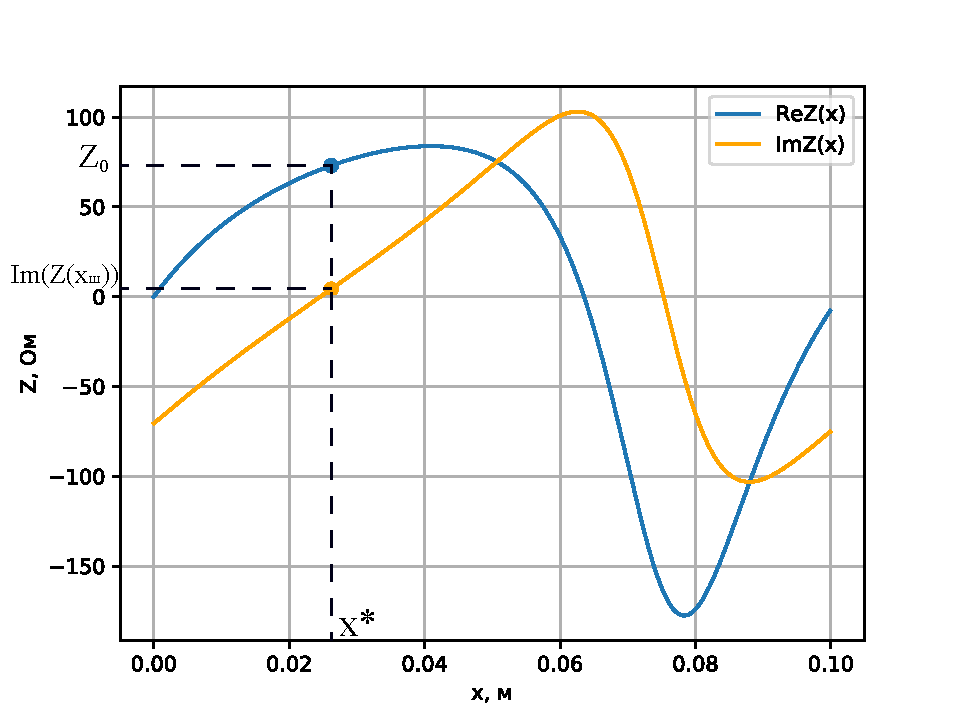
\includegraphics[width=1\linewidth]{2.pdf}}
\caption{Графічне визначення $x^*та X(x^*)$.}
\label{ris:image2}
\end{figure}


$Im(\dot{Z}(x_{\text{ш}}))=4.211 i$ --- опір шлейфа\\

$Z_{\text{ш}} = i\cdot Z_0 \cdot tg(k\cdot l_{\text{ш}})$\\

$l_{\text{ш}} = \dfrac{arctg(\dfrac{Z_{\text{ш}}}{Z_0})}{k} = 0.18$ см



\newpage
\clearpage
Висновок: у данній розрахунковій роботі було визначено параметри хвиль у довгих лініях. Знайшовши хвильовий опір лінії ми, при подальших обчисленнях, знехтували згасанням в лінії вважаючи що лінія у нас без втрат для спрощення розрахунків. Також був розрахований комплексний коефіцієнт відбивання, який включає в себе відношення амплітуд падаючої, відбитої хвиль та фазу відбивання. Виходячи з формул для розрахунку комплексного коефіцієнта відбивання видно, що він повністю визначається опором навантаження. Також визначили коефіцієнт стоячої хвилі (КСХ), який дорівнює відношенню максимальної і мінімальної амплітуд. Побудувано графіки розподілу амплітуд струму і напруги вздовж кабеля рис. \ref{ris:image1}. Потім було розраховане місце підключення та величину реактивності, необхідної для узгодження лінії з даним навантаженням. Для цього ми розглянули узгоджуючі пристрої, які створюють відбиту хвилю, рівну за амплітудою і протилежною за фазою відносно хвилі, для себе виявив, що графічний метод для знаходження опору узгоджувального пристрою та його місця підключення є зручнішим ніж чисельний.\\





%\clearpage
%\begin{center}
%\textbf{ДОДАТОК}
%\end{center}
%Для обрахунку всіх значень, графіків та поверхонь я написав програму на мові Python:\\
%\lstinputlisting[basicstyle=\ttfamily\footnotesize,language=Python]{rgr1.py}













\end{document}
